\documentclass[10pt]{article}
\usepackage{graphicx}
\usepackage{setspace}
\usepackage[margin=1.5in]{geometry}
\doublespacing
\title{Result Report on Finding Frequent Itemsets in a Large Dataset}
\date{2018-02-10}
\author{Zhengzhe Yang}


\begin{document}
	\pagenumbering{gobble}
	\maketitle
	\centerline{Team mates: Zhenzhe Yang}
	\newpage
	\pagenumbering{arabic}	
	
	\paragraph{\centerline{\textbf{Objective of this assignment}}}
	\hspace *{0.5 cm}In this assignment, we have to implement the Apriori algorithm to find the frequent itemsets with the minimum support count. In addition to obtaining the correct result, we need to optimize the performance of this algorithm to avoid excessive running time. To gain better performance, in this assignment I put the running time into the most priority and space usage to be second. Thus, it might use extra memory in order to run faster. 
	
	\paragraph{\centerline{\textbf{Optimization Methods}}}
	\hspace *{0.5 cm}The main problem that might cause the program to run forever is that we have to scan through the original dataset for multiple times to find its subsets and their number of occurrences. This takes ridiculously large amount of time, and it wouldn't finish for days when it comes to larger subsets, for example, finding subsets with 4 or 5 elements. Thus, we need to find a way to reduce the number of elements in the candidate sets, and more importantly, in the original dataset. According to the algorithm, we already figure out how to prune the candidate set. Recall that we build the candidate set by combining the elements in the last frequent itemset. If any of the subset of a newly generated candidate is not in the frequent itemset, we erase that from the candidate set, since there's no way for it to be frequent anymore, and we certainly don't need to check it. Now, for the original dataset, because we need to generate the subsets for every entry of in the dataset, it is going to be slow because there are 100,000 entries. Thus, I used a 3-d vector called $subset$ to hold all the subset for individual entry, and every time we generate new subsets, we replace every entry with the new subsets. In the first round, when we read in  the dataset, we find the 1-element frequent itemset, and update the subset with the found values. We also keep their counts with a hash map, which will be used to store all the subsets with their corresponding counts. Here, we will prune the $subset$ first to eliminate those who are not frequent. Next, we generate the subset based on the current subsets by joining them with the ones after them. Since they are organized in alphabetical order, we can easily generate next subsets with the previous subsets. Furthermore, when joining the current subsets, we can check in the hash map to see if they are frequent or not. If not, there is no need to put them into the newly generated subsets. We will not use the original dataset to generate subsets anymore. Instead, all the counting and operations will be done in the vector $subset$. By doing this, the dataset will become smaller and smaller, and the process of generating new subsets will become much more efficient, since we neglect those who are guaranteed not to be frequent, and we only traverse the dataset for once. However, I did notice that when generating the subsets with 2 elements, it takes unusual amount of time. This is probably because there are too many 2-element frequent itemset, and generating the subsets using previous subsets is not ideal because using loop to traverse $subset$ takes a long time, and the if-statement to check if the previous subset if frequent is not necessary, since the 1-element subset is pruned before. Thus, I used the old-fashioned way to generate the 2-element subsets, that is the backtracking. I currently use vectors as the key in my hash map, and with the Boost library, I can acquire reasonable hashing time. I believe the algorithm can be further optimized by using string as key in the hash map. Also, if we generate the output file using a single string, instead of writing to the output line by line, more time will be saved. 
	
	\paragraph{\centerline{\textbf{Results}}}
	\hspace *{0.5 cm}For minimum support count of 500, the time used to find the frequent itemset on the T10I4D100K dataset is around 14 seconds. For 1000, 8s. For 1500, 5s. For 2000, 4s. A plot is attached below. I also tested chess dataset, but for 2000 threshold it takes too much time. For a threshold of 2500, it took 167 seconds. For 3000, it took 2.9 seconds. 
	\begin{figure}[h!]
	\centering
		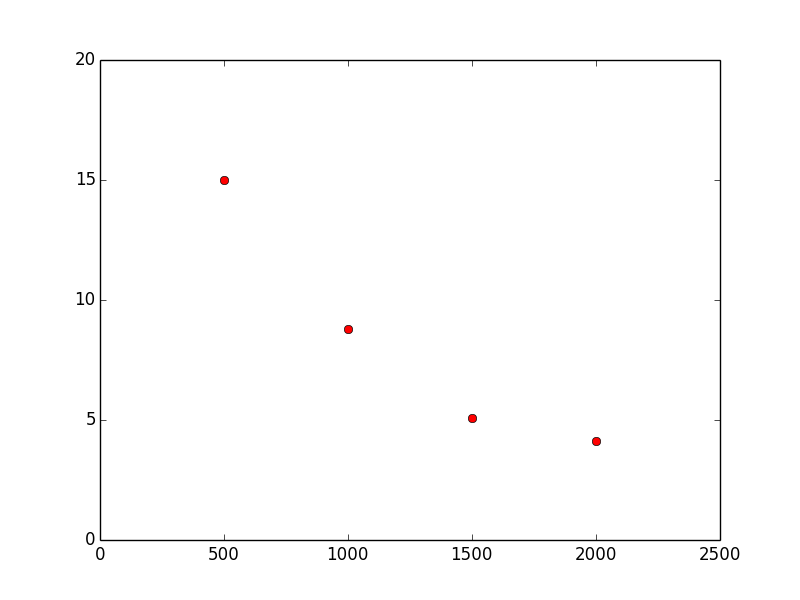
\includegraphics[width=0.5\textwidth]{figure_1}
	\end{figure}
	
	\paragraph{\centerline{\textbf{Refelection}}}
	\hspace *{0.5 cm}In this assignment, I learned that the techniques in data mining is not pure algorithm. Granted, algorithm is important, and a smart and efficient algorithm can improve the performance drastically. However, a more important aspect of data mining is data, including how we get the data and how we process the data to fit the algorithm ideally. With properly handled and processed data, we can acquire better speed and stability. Some algorithms is efficient with smaller datasets, but it couldn't perform very ideally on large dataset like the ones we use in this assignment. I believe the datasets are only going to be larger in real life problems. Therefore, I realize that there is still plenty of space for me to learn, especially if I want to engage in the industry of data.
\end{document}